\documentclass{polytech/polytech}

\typereport{prddi5}

\reportyear{2017-2018}
\title{Plateforme d'acquisition et de formatage temps réel multiflux TV Web}
\student[di5]{Romain}{ROUSSEAU}{romain.rousseau@etu.univ-tours.fr}
\academicsupervisor[di]{Mathieu}{DELALANDRE}{mathieu.delalandre@univ-tours.fr}


\resume{Ce projet consiste en l'élaboration d'une plateforme d'acquisition de flux TV Web en temps réel. L'objectif dans un premier temps consistera en l'affichage de plusieurs flux en simultané avant d'éventuellement faire évoluer l'application pour y faire figurer des éléments d'analyse d'images. Au travers de ce rapport, nous verrons la démarche, les objectifs liés à la mise en place d'une telle plateforme, l'architecture logicielle avec une structure en multi-threads, ainsi qu'un état de l'art sur ce domaine constante expansion et qui représente près de 80\% du trafic de données sur Internet.}

\motcle{Plateforme d'acquisition} 
\motcle{Flux de données} 
\motcle{Temps réel}
\motcle{Protocole de communication} 
\motcle{Télévision en ligne}


\abstract{This project consists in the making of acquisition platform of Live TV streams in real time. The first aim is to display multiple streams at the same time before evolving the platform to add elements of frame analysis. Through this document, we will see the approach, the goals link in the making of such a platform, the software architecture with a multi-threaded structure, as a state-of-the-art in this constantly evolving domain which represents almost 80\% of data traffic on the Internet.}

\keyword{Streaming Platform}
\keyword{Live Stream}
\keyword{Real Time}
\keyword{Communication Protocol}
\keyword{Online TV}


\posterblock{Contexte}{Le domaine du streaming est en constante évolution et représente près de 80\% de trafic de données sur le net.
	
	Alors qu’il existe de nombreux outils pour analyser les vidéos hors-ligne, il en existe très peu pour analyser les flux en direct, ce qui pourrait apporter de nouvelles possibilités dans de nombreux domaines du secteur des médias.}{images/illuStreaming}{Illustration sur le streaming}

\posterblock{Objectifs}{Le but est de réaliser une plateforme d’acquisition multi-flux TV Web. Dans un premier temps, le souhait est d’afficher en simultané plusieurs flux TV par le biais de la plateforme.
	
	Par la suite, nous pourrons implémenter des éléments de statistiques sur le flux arrivant ou bien de l’analyse d’images}{images/streamlink}{Aperçu de l'invite de commande pour le lancement de la plate-forme}

\posterblock{Fonctionnalités}{
	\begin{itemize}
		\item Sélection des chaînes désirées sur un fichier texte;
		\item Lancement de la plate-forme en ligne de commande;
		\item Affichage des flux en simultanés, avec gestion de la synchronisation.
	\end{itemize}
}{images/affichageFlux}{Exemple d'affichage de plusieurs chaînes en simultané}



\addbibresource{biblio.bib}

%%%%%%%%%%%%%%%%%%%%%%%%%%%%%%%%%%%%%%%%%%%%%%%%%%%%%%%%%%%%%%%%%%%%%%%%%%%%%%%%%%%%%%%%%%%%%%%%%%%
%%%%%%%%%%%%%%%%%%%%%%%%%%%%%%%%%%%%%%%%%%%%%%%%%%%%%%%%%%%%%%%%%%%%%%%%%%%%%%%%%%%%%%%%%%%%%%%%%%%

\begin{document}


\chapter*{Introduction}


Ce rapport traite du projet Recherche et Développement. Il s’étale sur l’ensemble de la cinquième année à l'école Polytech et représente une forme de synthèse des connaissances acquises lors des années d’études précédentes. Il permet de développer et d’approfondir son savoir sur un ou plusieurs champs de compétences spécifiques, afin de devenir un spécialiste du domaine choisi dans le cadre du projet. Ce travail est mené seul, sous la supervision d'un tuteur académique et avec l’aide d’un intervenant extérieur qui fait partie des initiateurs du sujet. Il permet ainsi de développer son autonomie en menant à bien un travail des prémices jusque, dans le meilleur des cas, à la production.

J’ai décidé de me consacrer à un sujet lié à un domaine en plein essor : le streaming. Ce sujet faisait partie de mes choix privilégiés lorsque j’ai vu la liste des sujets proposés. En effet, je regarde moi-même beaucoup de contenu audiovisuel par ce biais. J’ai pris pour habitude de regarder mes programmes télévisuelles préférés via mon ordinateur plutôt que par les usages traditionnelles avec une télévision depuis plusieurs années déjà, et il m’a paru intéressant de me pencher sur l’envers du décor et le fonctionnement de ces applications utilisées au quotidien par des milliers de personnes aujourd’hui.

Le but de ce projet est de mettre en \oe{}uvre une plate-forme permettant d'acquérir de multiples flux de chaînes de télévision. Le contexte, les acteurs et les objectifs seront détaillés dans la première partie de ce rapport. La deuxième partie sera consacrée à l'état de l'art sur la télévision et l'implantation générale des flux vidéos sur Internet ainsi qu'à la veille technologique pour la mise en place de la plate-forme, c'est-à-dire les différents protocoles utilisés, les bibliothèques d'acquisition à disposition, les serveurs distribuant les flux, etc.. La description générale du projet ainsi que les diverses fonctionnalités et caractéristiques présentes seront explicitées dans la troisième partie du document. La dernière section sera consacrée à la qualité du code et à la mise en place des tests autour de l'application. 

De nombreux documents complémentaires seront à disposition en annexes, notamment les diagrammes de Gantt, les diagrammes UML de la plate-forme, des schémas de l'interface, etc. Un guide d'utilisation de l'application est également présent en complément. Les sources du projet sont disponibles sur un dépôt GitHub à l'adresse suivante : \url{https://github.com/RomainR37/streamPlatform}.



\part{Contexte de la réalisation et cadre générale du projet}


Cette partie est consacrée au contexte générale de la réalisation, avec les enjeux, les acteurs impliqués ainsi que les objectifs fixés au démarrage. Nous verrons également les hypothèses auxquelles nous devrons faire face. Une section sur la base méthodologique utilisée et sur la gestion du projet sera également présente.

\section{Contexte, enjeux et acteurs}


Aujourd’hui, Internet est l’un des supports les plus répandus pour échanger et partager de l’information. En constante expansion, Internet est accessible par plus de la moitié de la population mondiale \cite{_chiffres_2017}. L’une des principales sources de transmissions d'informations sur Internet est la diffusion de contenu audio et vidéo, en effet plus de 75\% du trafic actuel est constitué de données vidéo et ce pourcentage augmentera jusqu’à plus de 80\% à l’horizon 2021 \cite{_cisco_2017}. La demande continue de prendre de l’ampleur au fil des années, les consommateurs réclamant des vidéos avec la meilleure qualité possible.

Avec cette évolution constante, la diffusion de contenu vidéo en ligne est devenue un enjeu majeur pour les entreprises s’installant sur Internet et en particulier pour celles spécialisées dans l’audio-visuel et les médias. Les plus grands groupes ont déjà tous développé des services permettant de voir leurs programmes en direct ou en différé sur Internet depuis plusieurs années déjà. De nos jours, elles sont utilisées couramment par le grand public (exemple avec la plateforme MyCanal du groupe Canal + qui compte 5 millions de visiteurs uniques par mois et près de 2 millions d’utilisateurs actifs \cite{sancerre_canal+_2017}) et les principaux acteurs du secteur tendent à vouloir élargir leur offre en se démarquant du modèle de la télévision traditionnelle.


\begin{figure}
	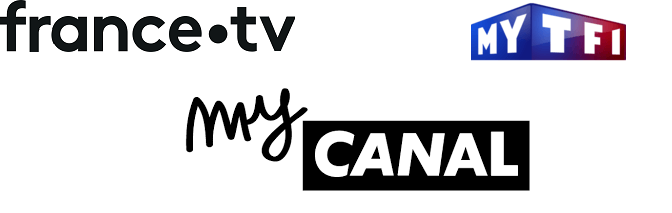
\includegraphics[scale=0.75]{images/exemple_sites.png}
	\caption{Exemples de plate-forme vidéo de grands groupes audio-visuels français}
	\label{fig:ex_plate-formes}
\end{figure}

Ils existent déjà de nombreux outils pour acquérir, stocker, traiter et indexer les flux de Web TV hors-ligne \cite{abduraman_tv_2012}. Cependant, la tendance actuelle est l’analyse de ces flux en continu, notamment par le biais de la détection de vidéos dupliquées \cite{liu_near-duplicate_2013}. Ce type d’analyse peut être appliqué à de nombreux domaines faisant l’objet d’enjeux majeurs pour les entreprises du secteur comme la protection de la propriété intellectuelle, la recommandation de vidéo, ou même le contrôle des vidéos.

Prenons un exemple d’analyse en continu qui est susceptible d’être utilisé dans le cadre de la télévision sur le web. Une entreprise souhaite vérifier si ces publicités sont bien passées à l’antenne. Par le biais de la détection vidéo, il serait possible en analysant le flux d’une chaîne souhaitée de savoir si la publicité est bien passée, à quel moment de la journée, sa fréquence sur un temps donné, et d’autres données pouvant intéresser l’entreprise. Récupérer ces informations avec une analyse manuelle du chaîne est laborieuse et coûteuse. Ainsi, la perspective d'un outil qui puisse analyser de multiples chaînes de télévision en simultané serait très intéressante pour des entreprises de publicités par exemple, mais aussi pour des institutions comme le Conseil Supérieur de l'Audiovisuel.

Ce projet a été initié par un ancien étudiant de Polytech Tours, M. Jordan NICOT qui, pour son projet libre lors de son dernier semestre, a réalisé un programme de traitement d’un flux RTSP. L’idée derrière son projet était de détecter si une chaîne de télévision diffusait des publicités ou non. Pour cela, la plateforme prenait un flux RTSP venant de son boîtier TV et effectuait un traitement d’images détecter l’apparition du jingle de publicité de la chaîne analysée. Le traitement était assez rudimentaire, puisqu’il consistait en l’analyse d’un encart de l’image dans lequel était écrit, avec une typographie particulière, le mot "publicités". L’analyse fonctionnait bien pour une à deux chaînes, mais pas pour toutes. Cependant, l’idée principale a été conservée, et sera exploitée lors de ce projet.

Ce sujet s’inscrit dans le cadre d’un projet de création de startup ImageStream engagé au niveau du Laboratoire d’Informatique Fondamentale de Tours (LIFAT), entre l’Université et le secteur privé. La mise en place future de cette collaboration dépendra de l'aboutissement du projet. 

\section{Objectifs}

L’objectif de ce projet est, à terme, de mettre en place une plateforme d’acquisition et de formatage en temps réel de flux TV Web. Le but est que cette plateforme soit adaptable afin que des éléments d’analyse et de traitements des données puissent être ajoutée par la suite. Pour le moment, nous nous contenterons d’afficher un ou plusieurs flux à l’écran en prenant en compte les capacités réseaux, et garantissant une synchronisation en horodatage des flux. À plus long terme, le but serait d'acquérir plusieurs dizaines de flux vidéo en simultané. L'intérêt par la suite serait de normaliser les images entrantes et de les analyser. En effet, la normalisation des images est nécessaire car les flux vidéos seront tirés de serveurs variés utilisant des protocoles, des résolutions, des débits d'images différentes. 

Le projet s’appuiera sur une partie des travaux de Jordan NICOT lors de son projet libre de l’année dernière. Le code ne sera pas repris dans son intégralité, le programme final de ce projet sera seulement inspiré de ses travaux, notamment de gestion et d’affichage du flux. La plate-forme sera conçue pour fonctionner dans l'enceinte de l'université, avec une connexion et une machine assez puissante pour avoir le moins de limitations techniques possibles.

\section{Hypothèses}

Le but de l’application est d’acquérir des flux TV retransmis sur le Web. Cependant, avec l’évolution des protocoles de streaming (voir \autoref{chap:diffusion_flux}), il devient de plus en plus compliqué de récupérer un flux TV pour un programme tiers. Les grandes plateformes d’hébergement de flux nécessitent souvent d’avoir un compte sur le site en question ou bien de souscrire un abonnement à un fournisseur de services. L’un des intérêts de l’application est qu’elle fonctionne pour toutes les chaînes accessibles gratuitement sur la télévision française par la TNT. Or, certaines d’entre elles pourraient être difficiles d’accès pour la plateforme.

L'une des solutions aux problèmes d'accessibilité des chaînes serait d'utiliser un programme externe comme Streamlink (que nous allons voir plus en détail dans la \autoref{sec:streamlink}) permettant d'exploiter des flux vidéos sur des sites. Nous avons opté pour cette solution bien que celle-ci ait néanmoins un inconvénient. Dans le cas où le programme n'est plus maintenu ou ne permet plus de récupérer les flux de certaines chaînes à cause de nouvelles protections, l'application ne fonctionnerait plus ou serait bridée par ce programme externe, indépendamment de notre structure. La meilleure solution à plus long terme serait de disposer d'une infrastructure professionnelle avec une autorisation des chaînes de télévision exploitées.


\section{Base méthodologique}


Lors des premières réunions du projet, nous avons opté pour une gestion de projet sous forme de cycle en V. En effet, la plate-forme ne nécessite pas une grande réactivité dans les demandes clients et l'expression des besoins est directement donnée par l'encadrant. Ceux-ci ne sont pas amenés à évoluer de façon drastique car ce ne sont pas des demandes provenant d'un client externe à l'école puisqu'il s'agit avant tout d'un projet interne à Polytech en premier lieu. 

Par ailleurs certaines étapes d'un cycle en V classique ont déjà été effectuées, la partie Expression des besoins ainsi que les spécifications fonctionnelles notamment, ce qui permet d'évoluer plus facilement à l'avenir et d'avoir une base pour aller plus vite dans les étapes suivantes. La première ébauche du diagramme de Gantt est disponible sur la \autoref{fig:gantt1}.

Malheureusement à l'issue du premier semestre, des retards se sont accumulés, en particulier sur la partie \'{E}tat de l'art et veille technologique. Les contours du projet et les modalités de développement étaient restés flous. Dès lors, un ajustement dans les objectifs et dans la gestion de projet était nécessaire. Ainsi, pour le deuxième semestre consacré au projet, nous avons opté pour une méthode Agile adaptée au peu de temps restant pour la finalisation du projet. Quatre sprints principaux se distinguaient, tous d'une durée de 2 à 4 semaines maximum:

\begin{itemize}
	\item Ajustement de l'état de l'art et de la veille technologique, avec l'ajout de plusieurs parties sur la télévision et sur des bibliothèques d'acquisition;
	\item \'{E}tude sur l'implantation des principales chaînes de télévision actuellement en France;
	\item Développement de l'application;
	\item Finalisation du rapport.
\end{itemize}

Le diagramme de Gantt ajusté pour le second semestre est disponible sur la \autoref{fig:gantt2}

Concernant la méthodologie de développement, les premières idées portaient sur une structure MVC (Modèle - Vue - Contrôleur) avec une partie Modèle qui se focalisera les objets représentant les flux vidéos, une partie Vue qui se concentrera sur l'affichage des fenêtres et sur l'interface en général, et enfin une partie Contrôleur qui fera la liaison entre les parties. Au fur et à mesure de l'avancement du projet, la partie Contrôleur a pris une place prépondérante par rapport aux autres car elle contrôle la redirection des flux, la création des objets et des fenêtres ainsi que le lancement des programmes externes. Les parties Modèle et Vue se contente donc de représenter les chaînes d'un côté et afficher les vidéos pour l'autre. Les détails de l'implémentation sont explicités dans le \autoref{chap:description}.


\part{\'{E}tat de l'art et Veille technologique}


\chapter{\'{E}tat de l'art sur la télévision}

\section{Diffusion d'une chaîne de télévision}


\begin{figure}
	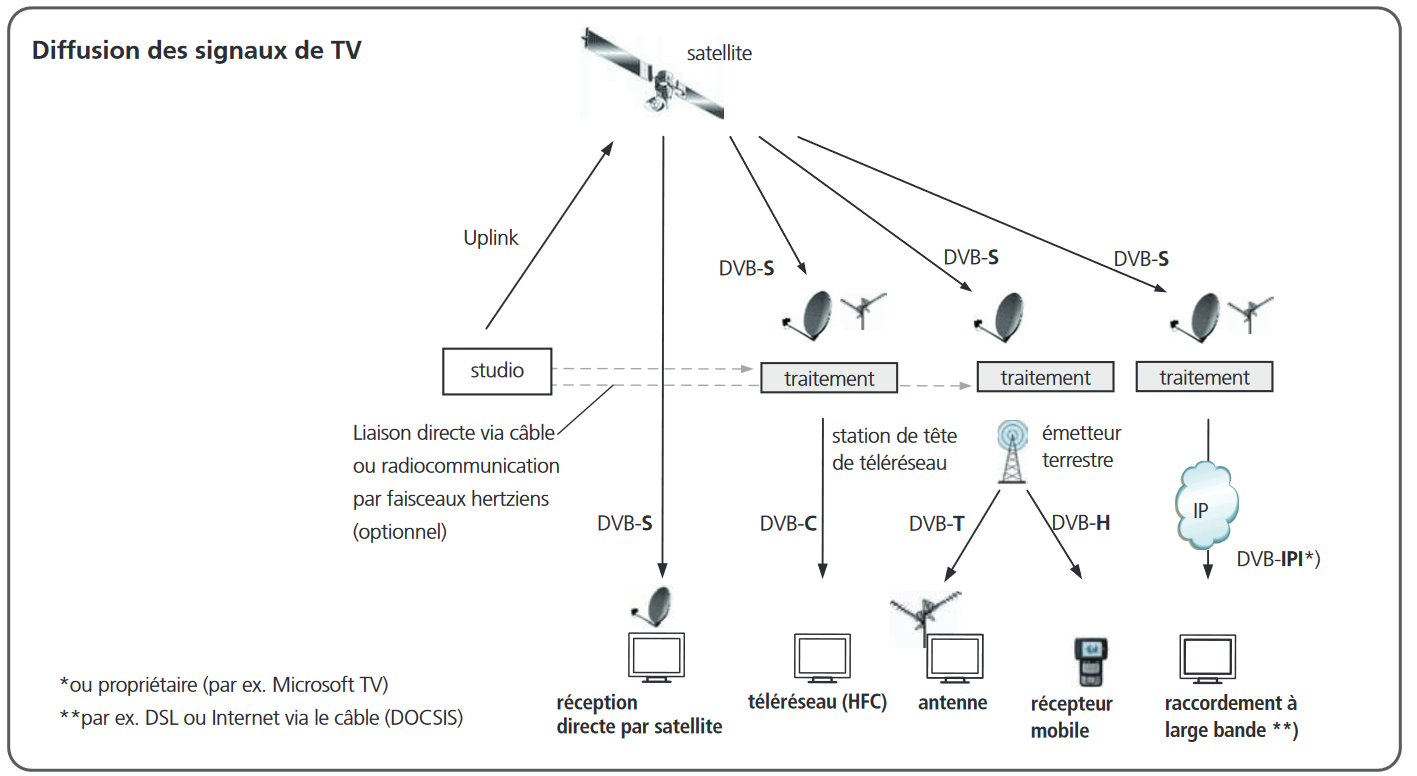
\includegraphics[scale=0.37]{images/diffusionTV.png}
	\caption{Schéma de diffusion d'une chaîne de télévision repris de l'article \cite{_diffusion_2018}}
	\label{fig:diffusionTV}
\end{figure}

\section{Réception de la télévision}

\subsection{Réception Hertzienne}

\subsection{Réception par satellite}

\subsection{Réception par câble}

\subsection{Service par contournement ou Over the Top (OTT)}


\chapter{La diffusion de flux en continu sur Internet}
\label{chap:diffusion_flux}

Dans la partie suivante, nous allons effectuer un tour d’horizon sur les flux en continu diffusés sur Internet ainsi que sur les possibilités actuelles en terme d’exploitation de données. Nous répondrons par la suite à plusieurs problématiques : comment les flux en continu ont émergé avec le développement d’Internet ? Quels sont les protocoles existants permettant de transmettre ces flux de données? Quelles librairies nous permettent d’acquérir et d’exploiter ces flux? Autant de questions auxquelles nous allons nous pencher dans les pages qui suivent.

Une parenthèse cependant concernant la suite de ce rapport, nous emploierons plusieurs termes pour définir la même notion, à savoir les flux de données en continu. Nous les nommerons flux, flux TV Web ou encore Streaming ou Streaming vidéo indifféremment. Le terme Streaming est tiré de l’anglais stream signifiant flot ou courant en français. Ce terme désigne aujourd’hui dans le langage courant la diffusion en continu sur Internet de contenus audio-visuels. Il existe différents types de données que l’on peut diffuser en continu sur une plateforme, mais nous nous focaliserons essentiellement sur les flux vidéo en continu, qui sont les bases de ce projet. Nous pouvons noter que les autres principes de flux de données comme le streaming audio que l’on peut retrouver sur des plateformes comme Spotify ou Deezer fonctionnent sur des bases similaires. Seules les données transférées diffèrent.

\section{Principe générale du \textit{streaming}}

La diffusion de flux en continu repose sur le principe d’une communication entre un client et un serveur. Les données sont mis à disposition sur un serveur et pour récupérer ses informations, le client envoie une requête qui lui communique les données souhaitées. Il existe deux types de lectures distincts \cite{_definition_2017} :

\begin{description}
	\item[Lecture Progressive] Cette forme de lecture est celle que l’on retrouve lorsque l’on regarde une vidéo sur un navigateur par exemple. Ici la vidéo est chargée, les données sont mises en cache par le client et la vidéo commence lorsqu’il y a assez de données en cache pour la commencer. La plupart du temps, le serveur propose plusieurs versions du même fichier avec des qualités différentes pour pouvoir s’adapter à la bande passante du client. C’est le principe que l’on retrouve pour le visionnage de vidéos Youtube par exemple.
	\item[Lecture en continu] Il s’agit de la forme de lecture qui nous intéresse pour ce projet. Ici, le contenu est diffusé au même rythme que la lecture. L’une des différences majeures est que le fichier envoyé par le serveur n’a pas de début et de fin définis comme pour un fichier statique. C’est un flot de données qui est envoyé au fur et à mesure au client.
\end{description}

Pour notre projet, nous nous intéresserons uniquement à la lecture en continu, qui est le principe des flux TV sur le Web. Et en particulier, l’un des aspects que nous rechercherons par la suite sur la diffusion de flux est le \textit{streaming} adapté ou \textit{Adaptive Streaming} en anglais que nous détaillerons dans la \autoref{sec:adaptative_streaming}.



\section{Genèse du \textit{streaming} vidéo et évolution au fil du temps}

Dans les années 1990, Internet commence à se démocratiser. Il est désormais accessible de s’acheter un ordinateur personnel pour un foyer lambda, quand les prix étaient encore très élevés dans les années 1980. L’élargissement de la bande passante ainsi que l’amélioration de l’accès aux réseaux accélèrent le développement d’Internet tel qu’on le connaît aujourd'hui. La possibilité de communiquer entre différents foyers et de diffuser des informations à travers le monde devient de plus en plus accessible par le biais de ce jeune Internet.

C’est en 1995 qu’apparaît la première diffusion audio en ligne en continu sur Internet. Il s’agissait d’un match de baseball proposé aux abonnés d’\textit{ESPNSportZone} en ligne. Ainsi, les abonnés de partout dans le monde ont pu suivre le match via un enregistrement radiophonique \cite{zambelli_history_2013}. La diffusion a été mise en place par une entreprise du nom de Progressive Network, qui plus tard, est devenu \textit{Real Network}.

Par la suite, les grands groupes informatiques de l’époque ont déployé tour à tour leurs solutions. Au début des années 2000, trois plateformes ont le monopole du streaming : \textit{Real Player} de \textit{Real Network}, \textit{Windows Media Player} de \textit{Microsoft} et \textit{Quicktime Player} de \textit{Apple}, avec chacun leurs propres technologies et protocoles de communication. Nous verrons par ailleurs le détail de certains de ces protocoles dans la \autoref{sec:protocoles}.

\begin{figure}
	
\includegraphics[scale=0.70]{images/logos_platform.png}
	\caption{Exemples de plate-forme populaire dans les années 2000}
	\label{fig:logoPlatform}
\end{figure}

Au fil des années, la concurrence évolue et devient de plus en plus rude. La technologie s’améliore et les anciennes plateformes dominantes deviennent rapidement obsolètes. Arrive au courant des années 2000 \textit{Adobe} et sa technologie \textit{Adode Flash} qui s’impose rapidement dans tous les foyers, si bien que l’add-on \textit{Flash Player} était installé sur 99\% des ordinateurs américains jusqu’en 2011 \cite{_chronique_streaming_2010}. Aujourd’hui, \textit{Flash Player} est devenu obsolète pour plusieurs raisons : tout d’abord, la technologie entraînait de nombreux bugs et failles de sécurité que déploraient la plupart des services l’utilisant, et ensuite, l’avènement de l’HTML5 sur les navigateurs a permis d’incruster une vidéo sur une page web sans avoir besoin de plug-ins particuliers. Tous ces problèmes concernant \textit{Flash} ont été listés notamment par Steve Jobs en personne en 2010 \cite{_thoughts_2010}, prônant par la même occasion le HTML5 et les nouvelles technologies émergentes. La page \textit{Flash} sera définitivement tournée dans les années qui viennent, avec l’annonce d’Adobe le 25 juillet 2017 qui prévoit son abandon définitif à l’horizon 2020 \cite{_flash_2017}.

La tendance aujourd’hui est aux nouveaux protocoles qui fonctionnent indépendamment de toutes installations de plug-ins ou de programmes pour fonctionner. C’est le cas par exemple du protocole HLS que nous observerons plus en détails dans la \autoref{subsec:newProto}. Par ailleurs, l’un des aspects importants de la diffusion en continu aujourd’hui est l’\textit{Adaptive Streaming} qui est exposé dans la partie suivante.

\section{Diffusion en flux adaptatif ou Adaptative Streaming}
\label{sec:adaptative_streaming}

La diffusion en flux adaptatif est une technique utilisée dans les protocoles modernes pour la diffusion de flux en direct. Elle consiste en l’adaptation de la qualité de l’image affichée en fonction de la bande-passante et de la capacité du processeur du client qui reçoit les données \cite{_adaptive_2017}. Il nécessite la présence d’un encodeur qui puisse recevoir le fichier que l’on souhaite transférer et qui le transmet au client avec plusieurs débits différents. Un schéma décrivant le fonctionnement lors d’une lecture d’un flux est à suivre :

\begin{figure}
	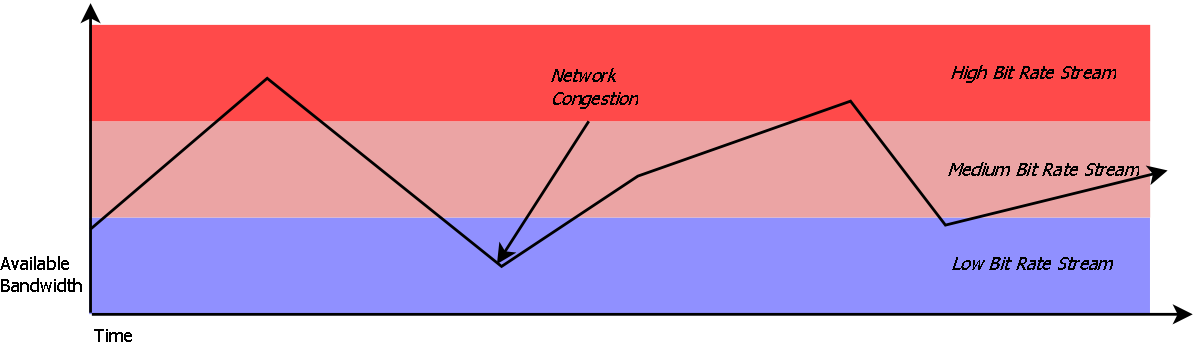
\includegraphics[scale=0.25]{images/Adaptive_streaming_overview.png}
	\caption{Schéma du fonctionnement de la diffusion en flux adaptatif (tiré de \cite{_adaptive_2017})}
	\label{fig:adaptive_bitrate}
\end{figure}

Le résultat induit un léger temps de chargement lors d’un changement de bande-passante mais un démarrage plus rapide de la lecture également. Ce principe est quasiment exclusif aux protocoles basés sur le HTTP et n’est pas adapté pour les protocoles plus anciens comme RTSP que nous verrons dans la partie \autoref{subsec:rtsp}. Ce type de diffusion est clairement celui-ci qui prend de l’ampleur et qui est particulièrement utilisé pour les Web TV.

La prochaine section détaillera les protocoles de communication les plus réputés dans le domaine du \textit{streaming} et leurs évolutions à travers le temps.


\section{Les protocoles}
\label{sec:protocoles}

Nous allons évoquer les différents protocoles de communication utilisables pour recevoir des flux de données en continu. Mais avant ça, il est important de définir ce qu’est un protocole de communication. Il s’agit d’un ensemble de règles définissant la procédure de communication sur un réseau \cite{_introduction_2017}. C’est par ce biais que les données sont communiquées et interprétées par la suite. Les protocoles que nous allons évoquer sont ceux qui ont été ou qui sont encore les plus utilisés pour le transfert de flux de données depuis l’apparition du streaming. Cependant, il en existe d’autres qui sont plus mineurs ou qui ont été moins présents sur le marché.

Les protocoles cités par la suite se trouvent sur la couche applicative de modèle OSI, cependant tous ces protocoles dépendent de la couche Transport et les protocoles de transport les plus utilisés pour la transmission de flux sont principalement le Transmission Control Protocol (TCP) et le User Datagram Protocol (UDP) \cite{_how_2016}. Le but du TCP est d’assurer le procédé de transmission des données, c’est-à-dire qu’on est sûr que toutes les données seront bien arrivées à destination. En effet, les paquets sont envoyés les uns après les autres, et si les premiers ne sont pas arrivés, les autres ne sont pas envoyés. Ce principe induit une possibilité de ralentissement, cependant il n’y aura aucune perte d’informations. Quant à l’UDP, la priorité est basée sur l’envoi d’informations en un minimum de temps. Ainsi, il est possible d’avoir des pertes d’informations lors de l’envoi des données mais la diffusion restera continu. De ce fait, pour la transmission en direct et pour avoir le moins de décalage, la préférence sera pour le UDP. Cependant, d’autres éléments peuvent rentrer en compte, notamment le fait que le TCP est utilisé dans de nombreux domaines sur Internet, et de ce fait, est moins susceptible d’être bloqué par un pare-feu que l’UDP. Le TCP sera malgré tout plus adapté pour les vidéos à la demande que pour la diffusion en direct.

Après avoir évoqué ces protocoles de transport, nous allons nous focaliser sur les protocoles de communication utilisables pour la diffusion de données en continu.


\subsection{HTTP}
\label{subsec:http}

Le protocole HTTP est un des protocoles les plus connus puisqu’il est à la base d’internet et des navigateurs Web. Il est aujourd’hui et de loin, le protocole le plus utilisé pour transférer des données média à la demande ou en continu \cite{_live_2017}. C’est avec ce biais notamment, et avec l’apparition d’HTML5, que les médias sont diffusés le plus facilement et le plus à même d’être à la disposition de tous.

Sans rentrer dans le fonctionnement détaillé du protocole, le principe d’HTTP est basé sur des requêtes échangées entre un client et un serveur. Il est générique, sans-état, et peut-être utilisé pour toute sorte de tâches différentes, de la navigation sur une page web à l’envoi de flux de données. C’est l’un des premiers protocoles à la base de la naissance d’Internet tel qu’il est aujourd’hui. Il est standardisé depuis 1996 \cite{fielding_hypertext_1996}, bien qu’utilisé depuis les origines du net dès 1990, et mis à jour régulièrement au cours des années avec les différents RFC publiés à propos du protocole. Il permet de transférer des textes, tout comme des données binaires et donc, tout type de médias divers et variés. Il utilise une structure sous forme d’URL pour décrire un objet. C’est ainsi que l’on peut remarquer que les adresses sur Internet utilisent toutes le protocole HTTP pour communiquer.

La tendance actuelle est de se séparer des autres protocoles de streaming courants pour revenir vers l’HTTP ou vers des protocoles basés sur ce dernier. Parmi les avantages, il y a notamment le fait de s’implémenter facilement, à moindre coût de par sa liberté d’exploitation, et la possibilité de faire de la diffusion en flux adaptatif comme vu dans la \autoref{sec:adaptative_streaming}.


Cette tendance vient d’une part, des failles de sécurité induits par certaines plateformes, et d’autre part, de l’avènement du HTML5. Le langage HTML est un format de données conçues pour représenter des pages web. Son principe repose sur des balises représentant un type de données qui s’affichera sur le navigateur. L’arrivée d’HTML5 en 2014 implique de nouvelles balises permettant d’implémenter des éléments multimédia directement sur la page \cite{_html5_2017}. Cela bouscule fondamentalement le marché, et induit une obsolescence de la quasi-totalité des extensions permettant de lire des vidéos diverses. En effet, auparavant, la lecture d’une vidéo sur un navigateur était possible uniquement via une extension comme \textit{Flash} ou encore \textit{Silverlight} par exemple.

Le HTTP étant le protocole qui permet d’envoyer des données HTML, l’impact du HTML5 a permis de remettre le protocole dans les premiers plans en ce qui concerne la diffusion de contenu et a aussi induit une explosion des nouveaux procédés, basés sur le HTTP, et prenant partie des nouvelles fonctionnalités mises à disposition par HTML5.

\begin{figure}
	
\includegraphics[scale=0.25]{images/html5logo}
	\caption{Logo du HTML5 qui a bousculé le marché du multimédia en ligne à son arrivée}
	\label{fig:html5logo}
\end{figure}

\subsection{RTSP et RTSP 2.0}
\label{subsec:rtsp}

Le protocole RTSP, acronyme de \textit{Real Time Streaming Protocol}, permet d’établir et de contrôler un ou plusieurs flux de données média en continu comme la vidéo et l’audio \cite{rtsp_1996}. Il a été l’un des protocoles pionniers dans la diffusion en continu et a été standardisé en avril 1998. Développé par \textit{RealNetworks} entre autres, il agit comme une sorte de télécommande sur les médias diffusés, avec des contrôles comme lecture, pause, arrêt ou encore enregistrer. Il utilise conjointement les protocoles de transport \textit{Real-time Transport Protocol} (RTP) et \textit{Real-time Control Protocol} pour envoyer les données média souhaitées. Quand RTP s’occupe de la transmission des données, RTCP se charge de transmettre des statistiques, des informations de qualité de service et aide également à la synchronisation en cas de multiples flux. RTSP est assez similaire dans sa structure à HTTP en terme de syntaxe et d’utilisation. Les deux protocoles utilisent une structure sous forme d’URL, pour le protocole RTSP, celle-ci commence par \textit{rtsp://}. À la différence du HTTP qui utilise par défaut le port 80 pour fonctionner, le port par défaut du RTSP est le 554. L’autre différence dans la conception cette fois est que, par rapport à l’HTTP qui est sans-état, RTSP fonctionne avec des états et permet ainsi de gérer différents flux sans problème.

L’un des points forts du protocole est sa flexibilité. En effet, le protocole peut échanger entre TCP et UDP pour promouvoir une meilleure expérience pour le client. Ce principe fonctionne aussi bien pour la diffusion en direct que pour les vidéos à la demande.

La version originale du protocole est devenue obsolète et a été remplacée par sa version 2.0 en décembre 2016 \cite{rao_real-time_2016}, bien que cette version ne soit pas rétro-compatible avec l’ancien protocole. Les ajustements apportés sont plus en phase avec la technologie et certaines modifications notamment dans les en-têtes des requêtes entraînent cette non-compatibilité.

De nombreux protocoles se sont inspirés de RTSP, notamment \textit{Microsoft} avec leur protocole propriétaire \textit{Microsoft Media Server}, rapidement devenu obsolète en 2003 et abandonné en 2008, et remplacé par RTSP sur les serveurs Windows.


\subsection{RTMP}

Le \textit{Real Time Messaging Protocol} était l’une des institutions du monde du streaming lorsque son développeur, \textit{Macromedia} qui en 2005 a été racheté par \textit{Adode Systems}, régnait sur le marché de la diffusion de données avec \textit{Flash Player}. C’est un protocole propriétaire qui permet de diffuser du contenu multimédia entre un serveur et un client possédant un lecteur Flash. Il existe différentes variantes de ce protocole comme RTMPE (pour Encrypted, qui signifie chiffré, ici en utilisant un mécanisme de sécurité propre à Adobe), RTMPS (pour Secure, en utilisant les procédés SSL/TLS) et RTMPT (qui est encaspulé dans des requêtes HTTP).

RTMP est basé sur le TCP, permettant ainsi une transmission des données fiable et une connexion stable. Il est aussi flexible, et permet d’envoyer des données audio, vidéo et même texte avec divers formats de fichiers vers différents appareils. Tout comme RTSP, le client peut contrôler le flux avec des commandes similaires pour gérer la lecture du flux.

L’un des avantages qu’il a toujours face aux protocoles modernes est son faible temps de latence, ce qui est d’une grande importance pour la diffusion en continu. De ce point de vue, il surpasse même les protocoles comme HTTP ou HLS encore de nos jours. L’autre atout majeur est sa capacité à être multi-plateforme. C’était l’une des grandes forces du protocole lorsqu’il régnait sur le marché dans les années 2000. Aujourd’hui cet argument n’est plus valable à cause de l’abandon progressif de l’extension Flash provoqué par l’arrivée d’HTML5. En effet, les dernières moutures de certains navigateurs ne sont plus compatibles avec Flash comme par exemple \textit{Firefox} ou \textit{Chrome}. Il était aussi auparavant disponible sur Android, ce qui n’est plus le cas depuis Android 4.0 sorti en 2011, dû notamment aux failles de sécurité du lecteur. Parmi les autres inconvénients, on retrouve l’instabilité en cas de bande passante changeante et l’absence de streaming en flux adaptatif.

Pour pallier à l’absence de flux adaptatif, Adobe a mis en place d’autres protocoles comme le HDS, basé sur l’HTTP.


\subsection{MPEG-DASH, HLS, HDS et les nouveaux protocoles basés sur HTTP}
\label{subsec:newProto}

Dans cette section, les protocoles cités sont ceux qui sont actuellement utilisés par les plateformes les plus connus. Tous ces protocoles sont basés sur l’HTTP vu dans la \autoref{subsec:http}, pour les raisons que nous avons déjà citées comme l’avènement du HTML5 ou le marché qui est concentré dans sa quasi-totalité sur ce procédé. Aussi, ils ont tous en commun d’être adaptés pour faire du streaming en flux adaptatif. Ils ont aussi la particularité de passer à travers les pare-feux et les serveurs proxy, étant donné qu’ils sont basés sur HTTP, ce qui n’est pas le cas des anciens protocoles de communication basés sur UDP, comme RTSP.

Le premier protocole que nous allons évoquer est celui qui est standardisé, à savoir la diffusion en flux adaptatif dynamique sur HTTP, couramment nommé MPEG-DASH \cite{_mpegdash_2017}. Il tient l’appellation MPEG du nom du groupe de travail \textit{Moving Picture Expert Group} qui est chargé des normes de compression, de traitement et de codage de fichiers multimédias. Ils ont par exemple à l’origine des différents fichiers de compression connus de tous comme le MP3 par exemple. Le MPEG-DASH est une technique de streaming adaptatif permettant d’envoyer des contenus média de haute-qualité à travers des serveurs HTTP. Il fait partie des solutions les plus populaires de par sa standardisation en avril 2012. Il fonctionne en divisant le contenu en plusieurs petites sections contenant un intervalle de temps du fichier complet. Chaque segment est disponible avec différents débits et ainsi, selon des facteurs déterminés par le client recevant les données, le contenu est envoyé avec le débit adapté de manière automatique. Les facteurs de détermination sont le vitesse de connexion, les capacités techniques de l’appareil mais aussi les préférences de l’utilisateur. Le but principal du standard est de proposer une diffusion avec le moins d’efforts de la machine pour n’importe quel format vers n’importe quel appareil. L’un de ces avantages par rapport à la concurrence réside dans la non-dépendance à un codec particulier. Un codec est un procédé qui encode et décode un flux de données pour le transférer par la suite. Là où les protocoles propriétaires ont tous un codec qui leur est propre MPEG-DASH peut s’adapter sur divers codecs différents.

Sous le même principe, reposent divers protocoles propriétaires, et notamment le plus connu, \textit{HTTP Live Streaming Protocol} (HLS). Développé par \textit{Apple} et initié en 2009, il utilise le même système que le MPEG-DASH, à savoir une division du fichier en plusieurs petites séquences de fichiers HTTP. Le protocole était destiné aux systèmes \textit{Apple} mais a depuis été étendu plus globalement. L’entreprise l’a documenté sous forme de RFC en 2015 et souhaite que le protocole devienne un standard reconnu. Il a été publié en Août 2017 et est en attente d’approbation pour le moment \cite{pantos_http_2017}. HLS présente l’avantage de prévenir les erreurs de flux en envoyant des extraits supplémentaires en cas de problèmes. Bien qu’il soit utilisé par des plateformes très utilisées (par exemple, \textit{MyCanal} la plateforme de \textit{Canal +}), il n’est pas recommandé pour effectuer des diffusions en direct, notamment en raison de son haut temps de latence lors de la transmission des données. Si on prend l’exemple de \textit{MyCanal}, il n’est pas rare d’avoir des décalages de plusieurs minutes par rapport à la diffusion télévisée. Le codec utilisé par le protocole est le M3U, qui nécessite l’utilisation de Javascript, supporté par les dernières versions des navigateurs web.

Parmi les autres protocoles propriétaires que l’on peut citer, il y \textit{HTTP Dynamic Streaming} (HDS), développé par \textit{Adobe}, qui fonctionne sur le même principe mais qui est appliqué au vidéo \textit{Flash}. De la même manière que HLS et MPEG-DASH, le serveur analyse la bande-passante du client et lui envoie les données qui lui correspondent le mieux. Cependant, ce protocole est voué à disparaître en même temps que l’extension \textit{Flash}.


\section{Les formats de fichiers utilisés}


\chapter{Les chaînes de TV sur Internet en France}


\section{Critères de recherche}


\section{Résultats de l'étude}


\section{Tendances observées}


\section{Un mot sur le copyright}


\chapter{Les bibliothèques et logiciels d'acquisition}

Pour notre plateforme, nous aurons besoin d’une bibliothèque qui puisse acquérir les flux de streaming afin de les traiter par la suite. Il existe de nombreuses librairies diverses et variées pour effectuer une acquisition de flux. Nous allons nous focaliser sur deux d’entre elles : VLC et FFMPEG.

\section{Les frameworks Windows (VfW, DirectShow, Media Foundation)}


\section{FFMPEG}

\begin{figure}
	
\includegraphics[scale=0.5]{images/ffmpeg}
	\caption{Logo de FFMPEG}
	\label{fig:logoffmpeg}
\end{figure}

FFMPEG est un ensemble de logiciels libres permettant d’acquérir, de convertir et d’enregistrer des flux vidéo et audio \cite{_ffmpeg_2017}. La première version du projet a été créée en 2000 et a depuis été reprise par de nombreux autres outils multimédia disponibles en ligne. Le projet est composé de plusieurs logiciels dont \textit{ffmpeg} qui est un outil en ligne de commande pour convertir des fichiers multimédia, \textit{ffserver} qui est un serveur streaming pour les diffusions en ligne, \textit{ffplay} qui est un lecteur utilisant les bibliothèques \textit{ffmpeg} et \textit{ffprobe} qui est un outil d’analyse de flux multimédia. En complément de ces outils, il existe également diverses bibliothèques qui sont proposées aux développeurs. Ces bibliothèques ont été rédigées en langage C et permettent de gérer diverses tâches liées aux flux de données. Ces outils proposés par FFMPEG sont libres et ont été utilisés dans de nombreux projets comme VLC par exemple.

Plus d’une centaines de fichiers et de protocoles sont pris en charge par FFMPEG, parmi eux, on retrouve les protocoles de communication que nous avons vu auparavant : HTTP, HLS, RTMP, RTP, etc. La liste des fichiers supportés est disponible \href{http://ffmpeg.org/general.html#Supported-File-Formats_002c-Codecs-or-Features}{ici}.

Parmi les logiciels, \textit{ffprobe} nous sera particulièrement utile pour afficher les statistiques liées aux flux de données que l’on souhaite visionner. Il offre tout un panel d’informations comme le codec, la disposition de l’affichage avec longueur et largeur de la fenêtre, mais surtout des chiffres sur le débit, le nombre d’images par seconde à l’affichage, le nombre d’images visionnées au total, et bien d’autres encore.


\section{libVLC et VLCJ}

\begin{figure}
	
\includegraphics[scale=0.5]{images/vlc-media-player-logo}
	\caption{Logo de la VideoLAN Organization}
	\label{fig:logovlc}
\end{figure}

LibVLC est une bibliothèque initiée par la \textit{VideoLAN Organization}, qui est à l’origine du lecteur multimédia VLC. \textit{VideoLAN} est une association à but non-lucrative qui développe et promeut des solutions libres pour le multimédia. Elle met à disposition de nombreuses bibliothèques et logiciels, dont le plus connu et le plus utilisé est \textit{VLC Media Player} \cite{_vlc:_2017}. Il s’agit d’un des lecteurs les plus réputés du marché dû à ses performances et ses possibilités pour lire la plupart des codecs audio ou vidéo. En effet, les codecs sont directement intégrés au logiciel grâce aux bibliothèques de FFMPEG.

LibVLC est rédigée en langage C, mais il existe de nombreux adaptations et frameworks reprenant la bibliothèque et qui sont adaptés à tout type de langage (C++, Java, Python, etc.). On peut retrouver la liste de ces bibliothèques sur ce \href{https://wiki.videolan.org/LibVLC/}{site}. Dans notre cas, on pourrait être amené à utiliser le framework VLCJ, qui permet d’importer un lecteur VLC dans une fenêtre JAVA.


\section{Streamlink}
\label{sec:streamlink}


\part{Description générale et analyse}


\chapter{Description générale}
\label{chap:description}

Le chapitre qui suit décrit ce que sera la plateforme, avec ces différentes spécifications. Nous détaillerons l’environnement du projet, les caractéristiques des utilisateurs, les fonctionnalités du système ainsi qu’une idée de ce que sera la structure générale de la plateforme.

Il est à noter que certains aspects ne sont pas encore fixés et sont susceptibles d’évoluer par la suite.

\section{Environnement du projet}

Ce projet sera testé sur les salles machines de l’école et branché sur le réseau de l’université. Il sera important de prendre en compte les capacités en terme de réseau de l’université afin de pouvoir acquérir de multiples flux sans encombre et sans problèmes de bande-passante.

\begin{figure}
	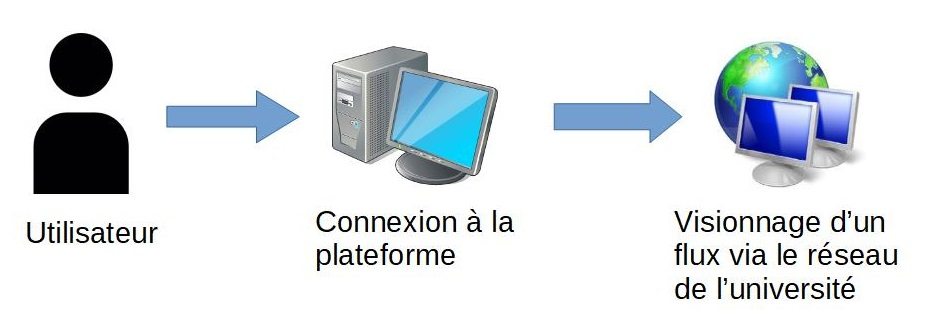
\includegraphics[scale=0.75]{images/environnement}
	\caption{Schéma de l'environnement du projet}
	\label{fig:environnement}
\end{figure}

Il est possible que certains flux soient bloqués par des pare-feux de l’université. Comme on l’a vu auparavant, cela pourrait se produire si on utilise des flux RTSP ou RTMP par exemple. Dans ce cas, il y aura une configuration de la machine à effectuer.

\section{Caractéristiques des utilisateurs}


Il n’y a ici qu’un seul type d’utilisateurs pour la plate-forme en ce qui concerne la première ébauche. La plate-forme n’est pas disposée à être accessible au grand public pour le moment. Un utilisateur classique aura accès à l’intégralité des fonctionnalités du système. Néanmoins, l’objectif est que la plateforme reste accessible facilement, quand bien même il serait restreint à un petit nombre d’utilisateurs. Dans le cas où la plateforme serait réutilisée et évoluée par la suite, il sera intéressant de disposer d’une interface simple et compréhensible, même si la personne n’est pas familière avec l’univers du streaming.

\section{Fonctionnalités du système}

Le système disposera de plusieurs fonctionnalités basiques que l’on peut retrouver dans le
diagramme de cas d’utilisation ci-dessous.

\begin{figure}
	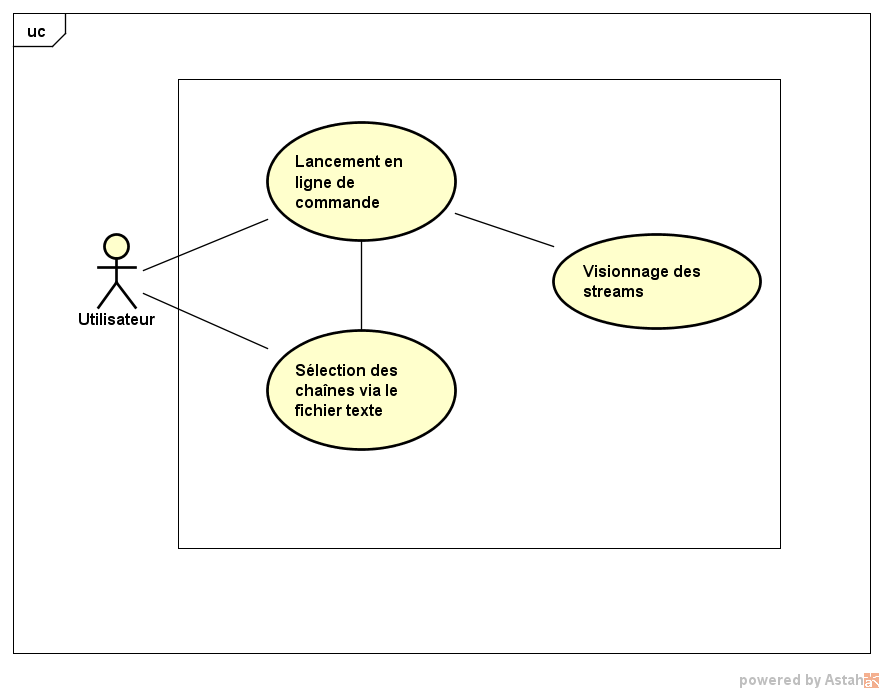
\includegraphics[scale=0.75]{images/UseCase2}
	\caption{Diagramme de cas d'utilisation}
	\label{fig:diagUseCase}
\end{figure}


\subsection{Séléction des chaînes via le fichier texte}

\subsection{Lancement en ligne de commande}

\subsection{Affichage des streams}

\section{Structure générale du système}


\subsection{La classe TVChannel}

\subsection{La classe MainLaunch}

\subsection{La classe MainControler}

\subsection{La classe StreamControler}

\subsection{La classe TextInputStreamControler}

\subsection{La classe StreamView}


\subsection{Lien entre les classes}


\chapter{Analyse des méthodes}



\part{Qualité de code et Tests de charges}


\chapter{Documentation et contrôle de qualité du code}


\section{Javadoc}


\section{Utilisation de SonarQube et SonarLint}

Pour le développement du site, nous nous sommes servis de l'outil de qualité de code \textit{SonarQube}. C'est un logiciel libre permettant de mesurer la qualité du code produit en se basant sur divers règles mises en place au préalable. Il peut détecter les bugs potentiels, les duplications de code, la couverture de code par les tests unitaires, et bien d'autres. Il supporte plus de 25 langages et s'adapte aux outils de build traditionnels (Ant, Maven, Gradle) ainsi qu'à certains IDE comme Eclipse. Il est aussi adaptable et personnalisable selon les besoins avec de nombreux plug-ins à disposition.

L'installation de SonarQube se fait très simplement. Il suffit de télécharger le programme, puis de lancer le script StartSonar.bat. Une instance de SonarQube sera lancée, et une fois que le message "\textit{SonarQube is up}" s'incrit sur la console comme on peut le voir sur la \autoref{fig:sonarcmd}, nous pouvons ouvrir la page du programme sur un navigateur. Par défaut, SonarQube utilise le port 9000 sur l'hôte local.


\begin{figure}
	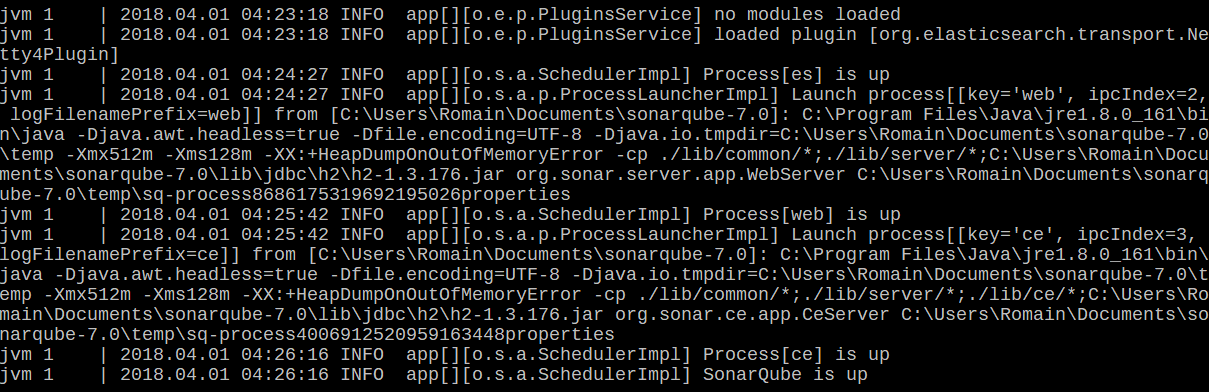
\includegraphics[scale=0.6]{sonarcmd.png}
	\caption{Lancement de l'instance SonarQube}
	\label{fig:sonarcmd}
\end{figure}


Maintenant que SonarQube est opérationnel, nous allons analyser notre projet. Dans un premier temps, nous regarderons l'application Angular. Dans notre cas, on souhaite que Sonar examine les fichiers \textit{typescript}. \'{E}tant donné que nous n'avons pas utilisé d'outils de build pour cette partie, nous avons installé un scanner sonar pour tout type de projet. Pour effectuer une analyse, il suffit de lancer depuis un terminal le script \textit{sonar-scanner} et de créer un fichier \textit{sonar-project.properties} comportant les détails concernant le projet, l'analyse s'effectuera par la suite. Le script va scanner tous les fichiers du dossier depuis lequel nous exécutons le programme et déterminera les éléments à modifier dans le code. Les résultats seront affichés dans l'instance SonarQube sur le navigateur internet.


Lors de notre première analyse sur l'application, nous avons eu les résultats suivants: 

\begin{figure}
	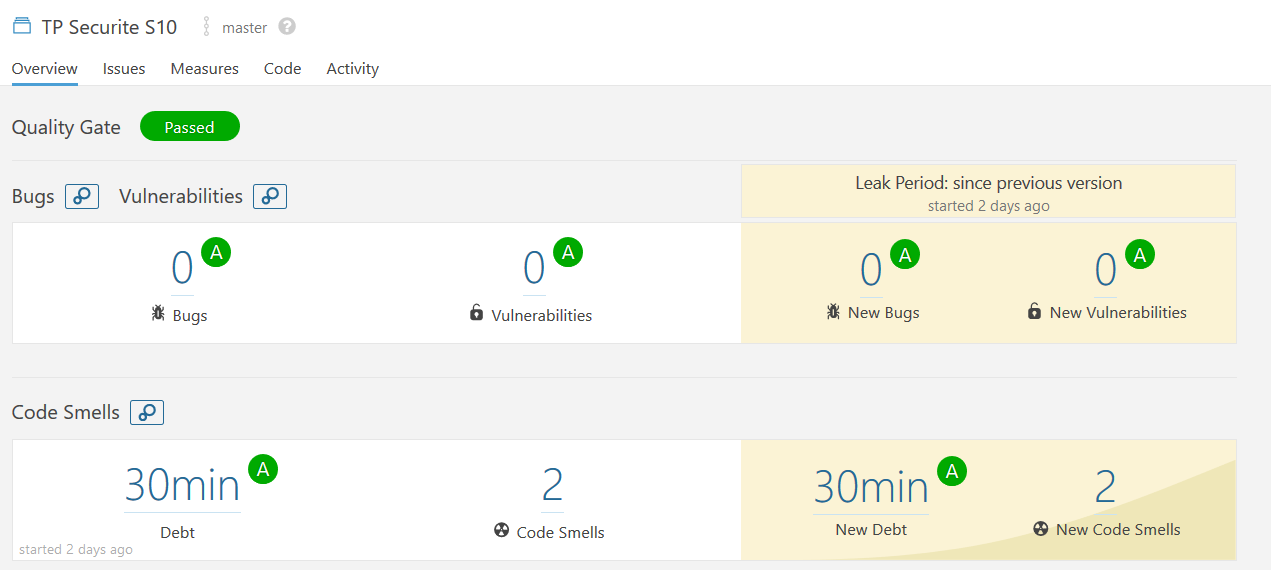
\includegraphics[scale=0.55]{sonarresult.png}
	\caption{Résultats de l'analyse Sonar}
	\label{fig:sonarresult}
\end{figure}

Nous pouvons remarquer que nous avons produit un code sans bug et sans vulnérabilités tout de suite, ce qui est déjà une très bonne chose. Il ne reste ainsi seulement qu'à corriger les deux erreurs détectées par Sonar pour avoir un code qui respecte les règles de Sonar. 


\chapter{Tests de charges}



\chapter*{Bilan et conclusion}

La première partie de ce projet aura abouti à une recherche approfondie sur les différentes solutions possibles pour la plateforme. Certaines questions restent cependant en suspens, et notamment la question des flux. Néanmoins, nous avons une idée de la structure future de l’application dont les spécifications nécessiteront d’être plus détaillées dans les jours à venir. Par la suite, l’ambition serait de terminer la conception architecturale de la plateforme dans les premières semaines de 2018 pour pouvoir entamer pleinement le développement jusqu’au mois de Mars.

En ce qui concerne la gestion du projet à mi-parcours, la phase de recherche a été assez laborieuse lors des premières semaines. En effet, le sujet est très vaste et documenté régulièrement depuis son apparition sur Internet. Or, si le domaine du streaming est vaste, il est en perpétuel évolution et a subi de grands chamboulements depuis l’arrivée d’HTML5 ces dernières années. Ainsi, il ne fallait pas se perdre parmi la pléiade de protocoles existants et aussi sélectionner ceux qui ne sont pas devenus obsolètes. Cette phase de recherche, bien que compliqué, n’en fut pas moins intéressante et m’a permis d’acquérir de nouvelles connaissances sur un domaine qui représente une proportion gigantesque de l’Internet tel qu’on l’utilise aujourd’hui. Mené à bien un projet sur un domaine crucial du secteur offre une motivation supplémentaire indéniable.


\appendix

\chapter{Interface Humain/Machine}

\chapter{Gestion de projet, diagramme de Gantt}


Ici, le diagramme de Gantt tel qu'il a été pensé à l'origine du projet. 

\begin{figure}
	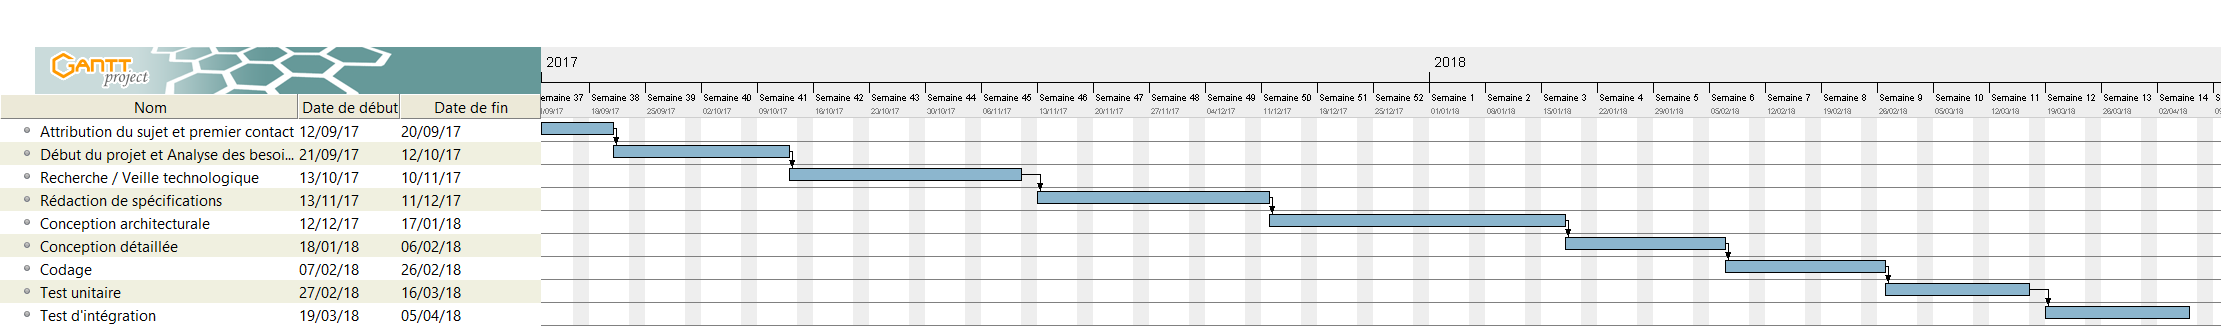
\includegraphics[scale=0.2]{images/Diagramme_PR&D}
	\caption{Diagramme de Gantt}
	\label{fig:gantt1}
\end{figure}


Ci-dessous, le diagramme de Gantt ajusté à l'issue du premier semestre.

\begin{figure}
	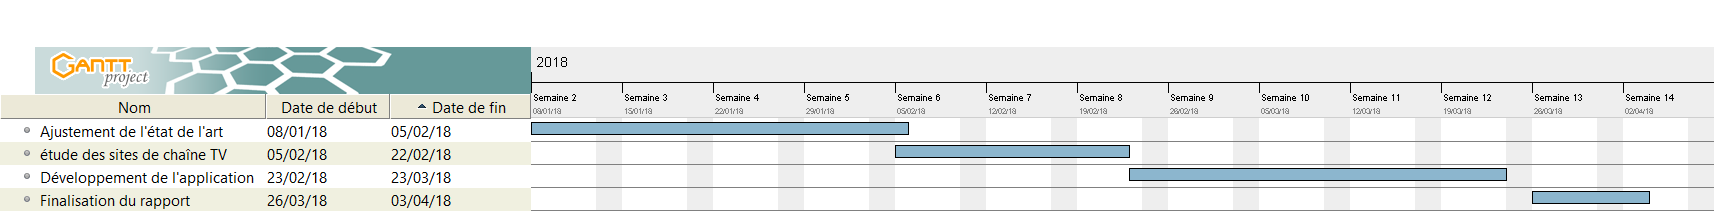
\includegraphics[scale=0.25]{images/Diagramme_PR&D2}
	\caption{Diagramme de Gantt ajusté à l'issu du premier semestre}
	\label{fig:gantt2}
\end{figure}


\chapter{Diagramme de classes}


\chapter{Diagramme de séquences}


\chapter{Guide d'installation et d'utilisation}


\section{Pré-requis}


La plateforme est destinée à fonctionner sur les machines de l’école. Il est nécessaire d'avoir une configuration réseau et matérielle solide si l'on souhaite faire fonctionner un maximum de chaînes en simultané sur l'application. La configuration minimale requise est la suivante :

\begin{itemize}
	\item Windows 7 Pro 64 bits
	\item Intel Xen CPU 3.06GHz
	\item 2 processeurs
	\item 4 Go de RAM
\end{itemize}


Pour la configuration réseau, la plateforme peut fonctionner sur un réseau Wi-Fi domicile mais la charge plafonne autour de 7 streams de qualité moyenne.


\section{Installations}

L'application nécessite plusieurs installations:

\subsection{Streamlink}

Streamlink est le logiciel en Python qui va prendre en charge les streams et qui va activer les flux à lire. Il existe plusieurs moyens de se procurer \textit{streamlink}, le plus simple est l'exécutable disponible à l'adresse : https://github.com/streamlink/streamlink/releases .

L'application fonctionne pour les versions 0.10.0 et supérieurs.

\subsection{VLC}

VLC est le logiciel permettant à l'application de visualiser les chaînes. Le programme  fonctionne avec la version 3.0.1 de VLC disponible à l'adresse suivante : \url{https://get.videolan.org/vlc/3.0.1/win64/vlc-3.0.1-win64.exe}


\subsection{Java Runtime Environment}

Le programme est un fichier jar qui fonctionne sur la version 8 de Java. Il est nécessaire pour le faire fonctionner de disposer du JRE 8 disponible à l'adresse : \url{www.oracle.com/technetwork/java/javase/downloads/jre8-downloads-2133155.html}


\section{Récupération du projet et fonctionnement}

Le projet se trouve sur le dépôt GitHub disponible à l'adresse suivante : \url{https://github.com/RomainR37/streamPlatform}

Une fois sur cette page, vous pouvez soit cloner le dépôt Git sur votre ordinateur, soit télécharger le dossier compressé en cliquant sur le bouton \textit{Clone or download} puis en sélectionnant son choix.

Après avoir récupérer le projet, vous pouvez l'exécuter en lancer une invit de commande Windows (en tapant Win+R au clavier puis \textit{cmd} dans le champ disponible). Une fois sur l'invit, dirigez vous vers le dossier du projet récupéré puis dans le dossier, allez dans le dossier \textit{target}. Il contient le fichier jar exécutable et un fichier texte exemple \textit{testStream.txt}. Pour lancer l'application avec le fichier \textit{testStream.txt} à disposition, la commande est la suivante : \javacode{java -jar streamPlatform-1.0.0-jar-with-dependencies.jar testStream.txt}. L'application se lancera.

\begin{figure}
	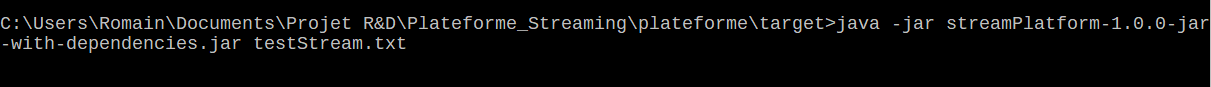
\includegraphics[scale=0.6]{images/cmdLancement.png}
	\caption{Commande de lancement du programme}
\end{figure}


\section{Fichier texte et syntaxe}

Il est possible de lancer l'application avec le fichier texte que l'on souhaite. Celui-ci pour fonctionner devra se situer dans le dossier \textit{target} également. Cependant le fichier doit respecter une convention de nommage. 


Une chaîne nécessite deux informations pour pouvoir fonctionner: son nom et l'adresse du site diffusant son stream. Dans le fichier texte que l'on veut lire, ces deux informations doivent transparaître séparées d'une tabulation. Vous pouvez voir l'exemple du fichier \textit{testStream.txt} ci-après:

\begin{figure}
	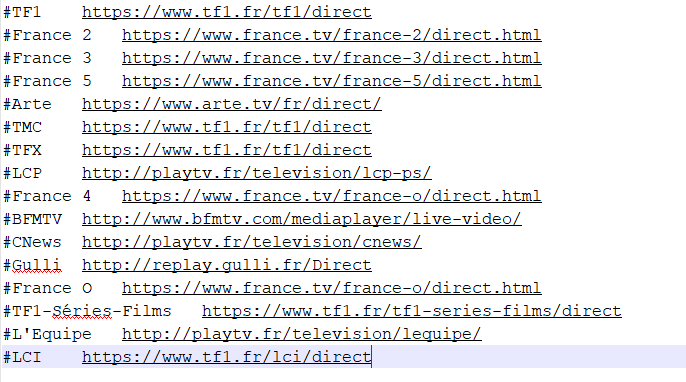
\includegraphics[scale=0.7]{images/testStream.png}
	\caption{Fichier texte exemple \textit{testStream}}
	\label{fig:fichier_texte}
\end{figure}

Ici sur la \autoref{fig:fichier_texte}, nous pouvons voir un \# avant une ligne. Il s'agit de la notation pour mettre une ligne en commentaire. Ainsi, le fichier \textit{testStream.txt} contient déjà une quinzaine de chaînes de télévision fonctionnelles, il suffit donc de supprimer les \# devant la chaîne que l'on veut visualiser. Néanmoins, il est possible de rajouter de nouvelles chaînes tant qu'elle respecte la convention. 

Certaines chaînes ne fonctionnent pas avec streamlink, et ne sont donc pas disponibles sur l'application. Par exemple, la version 0.11.0 de streamlink ne prend pas en charge les chaînes diffusées sur Dailymotion. Le problème sera sans doute réglé dans les prochaines versions ce qui rajoutera de nouvelles chaînes disponibles au visionnage. 


\section{Problèmes pouvant survenir}



\subsection{Pare-feu de Windows}

Un message du firewall peut apparaître au lancement de l'application. Cela est dû au script Python lancé par Streamlink. Il suffit que le firewall accepte les scripts pour que le fonctionnement se passe correctement. 


\subsection{Problèmes d'affichage}

Sur certaines machines, et en particulier sur les machines virtuelles de l'école, il est possible de constater des problèmes d'affichage des chaînes. On peut voir en effet sur des streams de bonne qualité, des problèmes au niveau des contours sur l'image (comme sur la \autoref{fig:pbAffichage}, en particulier à droite de l'image).


\begin{figure}
	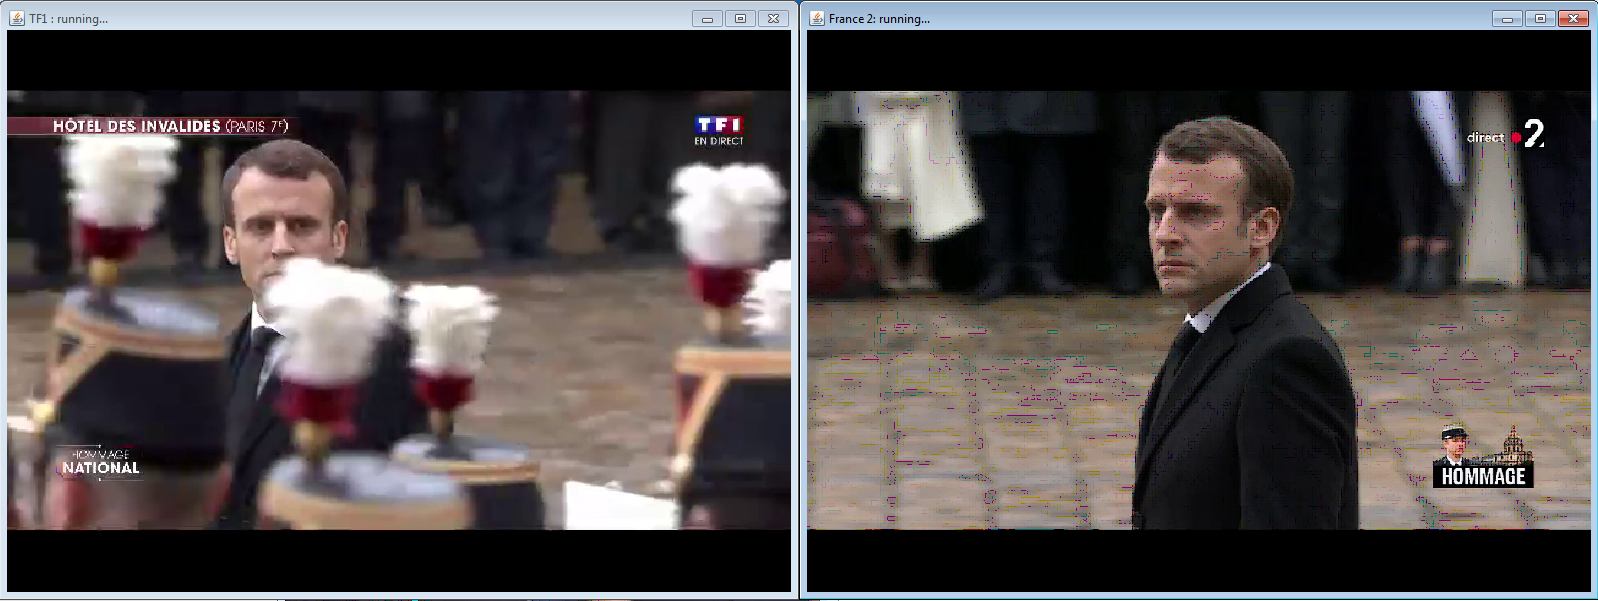
\includegraphics[scale=0.75]{images/imageQualite.png}
	\caption{Exemple de problèmes d'affichage}
	\label{fig:pbAffichage}
\end{figure}


Ces problèmes peuvent venir des configurations graphiques de la machine, notamment de DirectX. Néanmoins, lors des tests effectués sur machines Windows 10, il n'y avait aucun problème d'affichage, donc cela pourrait être des anciens systèmes Windows également.


\end{document}